\externaldocument[I-]{MaxHughesThesis}

After the half-life measurement was completed, the next step was to use the shape of the spectrum to deduce Fierz term. 
In order to get a measurement of the Fierz term, the spectrum shape needed to be carefully described.
In addtion to all the theoretical corrections, the effect of bremstrahlung and the effieciency of the detectors needed to be accounted for.
The way this was done was with a GEANT4 simulation.

\section{GEANT4 Monte Carlo}
The corrected beta decay spectrum was fed as input to a Monte Carlo.
The program used to model the detectors was GEANT4.
In order to use the program, a model of the detector set-up and the initial energies of the primary particles need to be introduced.  

\subsection{Detector Geometry}
The geometry of the detector set-up was programmed into the simulation.
The implant detector was modeled as a square prism of CsI.
The rectangular prism was 9.76 cm deep with a 5 cm square base.
The front edge implant detector was put at the center of the simulation.
The aluminum sheath and MgO layer was not simulated for the implant detector.

The four large gamma detectors also square prisms.
The active volume was 79.5 mm square and 76.2 mm deep.
It was also made of CsI.
There was a 2 mm dead layer of vacuum around the detector.
Above this dead layer, a 1.5 mm laywer of MgO was added.
On top of this, the can of aluminum, 1 mm thick, was added into the simulation.

The four large gamma detectors were arranged into a square around the implant detector.
Each square base of the gamma detectors was centered one inch upstream from the face of the implant detector.
This modeled how the implant detector was recessed in the experiment.

A visualization of the CsI crystals in GEANT4 is shown in figure \ref{gif:GEANT4Det}

\begin{figure}[!htb]
	\centerline{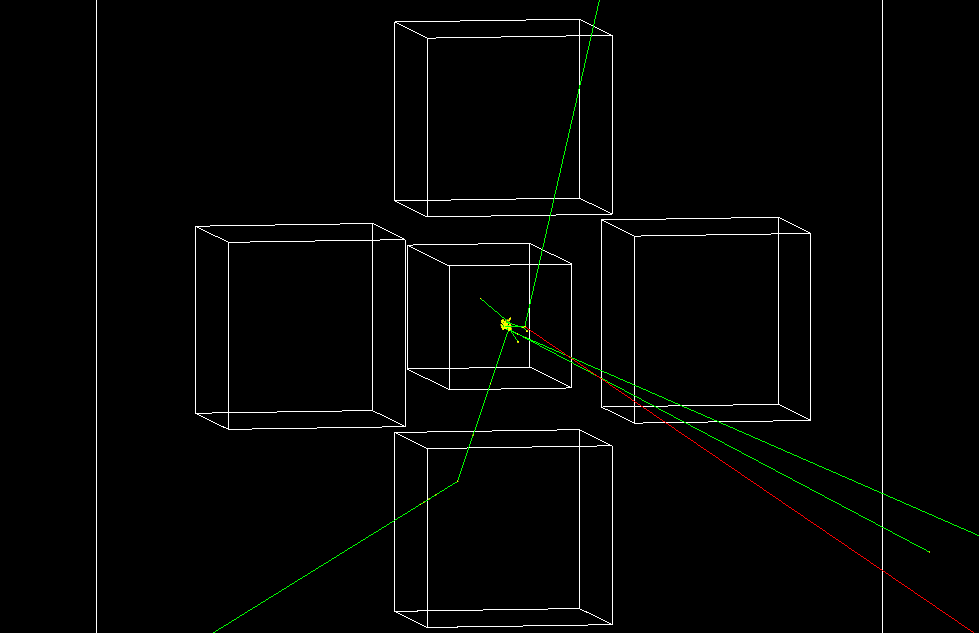
\includegraphics[width=0.78\textwidth]{GEANT4WithoutAl.png}}
	\caption{The detector geometry inside GEANT4}
	\label{fig:GEANT4Det}
\end{figure}

\subsection{Source Definition}
The next step was to define a region inside the implant detector.
This region was where the gamma and beta particles orignated from.
The depth of the region was calculated using LISE++, a ion optics code.
The verticle and horizontal size of the region was calulated by using the PPAC measurement and an ion optics simulation.
This size was 0.4 mm deep, 3.5 mm wide, and 3.6 mm tall.
The source was implanted 1.156 cm into the detector.

\subsection{Primary Particle Definitions}
There were three primary particles generated.
Two were photons and one was an electron.
All three particles had an isotropic angular distribution, and would propogate in different directions.

The first particle was an electron. 
This selected the point in the source region.
In order to generate the correct energy for this electron, the following process was used.
First, all the corrections described in chapter \ref{ch:theory} were multiplied with equation \ref{eq:phase_space}.
This resulting function was evaluated at 1024 evenly space points from 0 keV to the end point energy.
This list of 1024 points was fed into GEANT4 as a histogram, as GEANT4 can only take a histogram of up to 1024 bins. 
Linear interpolation was used to make this histogram back into a smooth function.
This is not exactly a histogram of the beta energy spectrum.
The original function was fit to the generated beta energies, and no distortions were generated using this procedure.

The next photon was the 1.6336 MeV photon from the $^{20}$F decay.
The energy of this photon was not changed.

The last photon was to account for the inner bremsstrahlung.
The radiative correction used to generate the electron energy was the formala that assumes all real photon energy is absorbed (equation \ref{eq:fayansrad}).
After the electron energy is generated, the formula describing the energy spectrum of the inner bremsstrahlung photons is generated. 
This spectrum is written out in equation \ref{eq:KUB}. % Add KUB again here? Probably.
Further discussion of this formula is found in the theory chapter.
A cutoff of 50 keV is imposed to the formula, as it has a singularity at zero photon energy.
In addition, with this geometry, all photon energies below 100 keV and absorbed.
Then, the formula is numerical integrated from 50 keV to the electron energy over X steps using the trapezoidal rule.
This is the total probablity that an electron emits a KUB photon.
This number is compared to a random number from 0 to 1.
If the random number is below the integral, the inner bremsstrahlung energy spectrum is sampled.
The algorithm used for this sampling is the van Neumann method \cite{neu51}.
The sampled energy is given to the third primary particle.
If the random number is more than the integral, the third primary particle is given an energy of 0 keV.
The energy of the electron is reduced accordingly.

The two photons had their initial points moved to match that of the electrons.
All three particles were then free to propagate throug the detectors.

\section{Particle Propogation}  

\section{MC Output}
The particles were tracked and the energy deposited in each detector summed up.
The energy deposited in the implant detector was further seperated into two parts:
Energy from the  electron and the inner bremstrahlung photon.
Energy from the 1.6336 MeV photon
After the energies of the particles reached a certain threshold, the simulation of one decay was finished.
All the energies deposited into each of the detectors was summed up and saved as an event in a ROOT tree.
Then, the process was repeated.
A new location inside the region was generated and another decay generated.

In order to get to get the necessary statistics, 2 * 10$^{9}$ events had to be generated. 
This initially took 7 days to run. 
In order to decrease the time it took to run, the range cuts on the gamma rays were changed.
The range cuts were changed from 5 $\mu$m to 5 mm for all gamma rays.
The range cuts for other particles stayed at 5 $\mu$m.

\section{Simulation Devolopment}
Initially,  

